\chapter{Dynamic Active Curricula}\label{ch:DAC}
The results laid out in Chapter \ref{ch:BootstrappedActiveCurricula} suggest that generalization performance can indeed be improved through the use of a learning curriculum, and that using active learning approaches to score which training samples are hard or difficult can be an effective way of automatically constructing such curricula without manually analysing the training samples. The disadvantage with the BAC method from Chapter \ref{ch:BootstrappedActiveCurricula} however is that it is necessary to first train a `baseline' model that can be used to derive a curriculum based on which samples it is uncertain about classifying. While in some cases this may not be too significant a computational burden, it effectively doubles the overall training time, motivating the approach laid out in this section. Specifically, we wish to investigate methods that can dynamically construct a curriculum throughout training, without needed to reference another model. We do this by calculating the prrediction uncertainty of the curriculum model itself over the training samples throughout training, using the uncertainty scores to construct dynamic curricula which adapt to the changing parameterisation of the model. If successful, these methods should lead to model performance which beats a the benchmark test set performance of a baseline model trained on the entire training set without a curriuclum, and hopefully will achieve results similar to those achieved by the bootstrapped active curricula from Chapter \ref{ch:BootstrappedActiveCurricula}.
\section{Curriculum Construction}
\subsection{Dynamic Task Curricula (DTC)}\label{sec:DTC}
The first dynamic curriculum method we test we term \textit{dynamic task curricula}; this approach is very similar to that of the BAC method laid out in Chapter \ref{ch:BootstrappedActiveCurricula}, however instead of constructing tasks based on the uncertainty scores of a fully trained `baseline' model, tasks are constructed dynamically using the uncertainty of the curriculum model itself throughout training. To do this, we calculate the model's uncertainty in predicting the classes of the training samples in the full training set $\mathcal{T}$ using the AADT function \ref{BAC_AADT} (or another active learning uncertainty measure) at the beginning of every epoch\footnote{With the exception of the first training epoch which uses the entire training set in order to allow the model to begin to calibrate to the problem.}, then ranking the training samples by the the model's uncertainty. We then split the training data into separate tasks, with the first task consisting of the first $\frac{1}{T}$ samples where $T$ is the chosen number of tasks. At the start of each epoch, we will obtain a new set of ordered tasks, $\mathcal{T}_i^1, \mathcal{T}_i^2,...,\mathcal{T}_i^T$, where $i$ is the current epoch, and $T$ is the chosen number of tasks. Training is divided into $T$ phases, such that, during epoch $i$ of phase $t$, the model is trained on a training set consisting of $\mathcal{T}_i^1 \cup \mathcal{T}_i^2 \cup ... \cup \mathcal{T}_j^t$, where $t$ denotes the current training phase.The final training phase will therefore consist of training on the full training set, as $\mathcal{T} = \mathcal{T}_i^1 \cup \mathcal{T}_i^2 \cup ... \cup \mathcal{T}_i^T, \forall  i$. As in the BAC curriculum method from Chapter \ref{ch:BootstrappedActiveCurricula}, we normalise the number of parameter updates in each phase by scaling the number of epochs relative to the number of samples used to train in that phase. Similarly to Equation \ref{eq:BAC_Epochs}, the number of epochs in training phase $t$ is set as follows:
\begin{equation}\label{eq:DTC_Epochs}
NumEpochs^{t} =\floor{ \frac{TotalEpochs}{t}}
\end{equation}
where $TotalEpochs$ is the number of epochs the model would need to be trained for on the whole training set in order to achieve the same number of parameter updates as the DTC curriculum method.

Note that we can rank the samples both from low to high uncertainty or from high to low uncertainty; in the low to high case the first tasks will contain samples about which the model is confident in predicting, corresponding to dynamically constructing an `easy to hard' curriculum. Alternatively, ranking the samples from high to low uncertainty will produce a curriculum more similar to an active learning approach, focusing on training the model on areas of the input space that it is more uncertain about classifying. While the latter method may contradict some of the usual motivations for curriculum learning \cite{Bengio2009}, we would still argue that the hard to easy approach still qualifies as a curriculum method, and may be appropriate in instances where the model already has achieved a high level of expertise in the problem, and improvements are arguably more likely to be made by studying harder samples than easy ones.  We therefore have two variations of the Dynamic Task Curriculum method; `Easy to Hard' DTC and `Hard to Easy' DTC. This approach is similar to that of \textit{Self-Paced Learning} \cite{kumar2010self}, where they apply a similar approach with a latent SSVM model \cite{felzenszwalb2008discriminatively}, however they implement their method by introducing a regularization term reflecting the difficulty of each sample into the objective function of the model, as opposed to employing an actual curriculum. As the model parameters are initialised randomly, it would be inappropriate to infer model uncertainty before the first epoch, as such, the first epoch is trained using the whole training set, and the use of the curriculum method begins starting with the second epoch.  Pseudocode for the DTC method is given in section \ref{sec:DTCPseudocode}.

\subsubsection{Pseudocode for the DTC curriculum}\label{sec:DTCPseudocode}
Pseudocode for the dynamic task curriculum method (assuming the use of the AADT uncertainty function and an easy to hard curriculum):
\begin{algorithmic}
\REQUIRE $Num\_Epochs$
\REQUIRE $Num\_Tasks$
\REQUIRE $\mathcal{T}$ \COMMENT{Full training set on input-label pairs}
\REQUIRE $\theta_{curriculum}$ \COMMENT{Model to be trained with the curriculum}
\FOR {$i=1$ to $Num\_Epochs$}
\STATE $TrainingPhase = \floor{\frac{i*Num\_Tasks}{Num\_Epochs}}$
\STATE $PhaseEpochScale = \frac{Num\_Tasks}{TrainingPhase}$
\FOR {$PhaseEpochScale$}
\STATE $\mathbf{s}^{\theta_{curriculum}} = AADT_{\theta_{curriculum}}(\mathcal{T})$
\STATE $\mathcal{T}_{\mathbf{s}^{\theta_{curriculum}}} = \mathcal{T}, \text{sorted by } \mathbf{s}^{\theta_{curriculum}} \text{ (descending order)}$ 
\STATE $Num\_Samples = |\mathcal{T}_{\mathbf{s}^{\theta_{curriculum}}}|$
\FOR {$t=0$ to $Num\_Tasks$}
\STATE $TaskStartIndex = Num\_Samples*\frac{t}{Num\_Tasks} $
\STATE $TaskEndIndex = Num\_Samples*\frac{t+1}{Num\_Tasks} $
\STATE $\mathcal{T}^{t}_{\mathbf{s}^{\theta_{curriculum}}} = \mathcal{T}_{\mathbf{s}^{\theta_{curriculum}}}[TaskStartIndex:TaskEndIndex,:] $
\ENDFOR
\STATE $\text{train }  \theta_{curriculum} \text{ on training set } \mathcal{T}^{0:TrainingPhase}_{\mathbf{s}^{\theta_{curriculum}}} $
\ENDFOR
\ENDFOR
\end{algorithmic}


\subsection{Dynamic Sampling Curricula (DSC)}
The second dynamic curriculum construction method we test is \textit{Dynamic Sampling Curricula (DSC)}; one of the potential problems with some curriculum and active learning methods is that of \textit{diversity} \cite{jiang2014self}. Diversity refers to how well the whole training set is represented in the samples used to train the model; if a sample selection method is extremely un-diverse then it may end up selecting only a very small selection of the training samples, leading to the model not training on a suitably broad set of training samples, resulting in high generalization error \cite{jiang2014self}. One way to approach this problem is to avoid deterministic methods of selecting training examples, and instead sample from the training data using some probability distribution. Mini-batch stochastic gradient descent is one such method, sampling batches of examples from the training data using a uniform probability distribution, however by varying the sampling distribution away from a uniform distribution we can bias training towards different samples, resulting in them being selected more or less often than others. 

We implement the DSC curriculum method by biasing the sampling probability proportionally to the model uncertainty in predicting the labels of the sample. In particular, at the start of every epoch we use an uncertainty function (for example the AADT function introduced in \ref{BAC_AADT}) to infer the model's current uncertainty in predicting the labels of the training data, giving $\mathbf{s}^{\theta_{curriculum}}$, a vector of $N$ scores as in Equation \ref{eq:BAC_S}, where $N$ is the number of samples in the full training set $\mathcal{T}$ and the $i^{th}$ element of $\mathbf{s}$ corresponds to the output of the AADT function for the $i^{th}$ training input. We then pass the vector of scores through the softmax function \cite{Theodoridis2009}, effectively transforming the scores into probabilities that can be used as the sampling probability distribution. For example, assuming the uncertainty function used is the AADT function, we can set:
\begin{equation}\label{eq:DSC_Prob}
\tilde{p_j}(x_i | \theta_j) = \frac{exp(\frac{AADT_{\theta_j}(x_i)}{\tau})}{\sum_{k}^{N} exp(\frac{AADT_{\theta_j}(x_k)}{\tau})}
\end{equation}
where $\theta_j$ is the model being trained with the curriculum after $j-1$ epochs, $\tilde{p_j}(x_i | \theta)$ is the sampling probability of training sample $i$ in the $j^{th}$ training epoch, and $\tau$ is the softmax temperature parameter that can be set as a hyperparameter or tuned each epoch to achieve a target diversity level in the sampling probability. The sampling probability is updated at the start of each epoch and training proceeds as with normal mini-batch stochastic gradient descent, using the sampling probabilities calculated in Equation \ref{eq:DSC_Prob} to sample from the entire training set. As we wish to bias training towards certain certain/uncertain samples, we also do not follow the typical SGD practice of sampling without replacement, instead sampling with replacement. As sampling with replacement implies that some samples will probably not be used in every epoch, this in effect introduces a stochastic curriculum where, instead of removing samples entirely from certain training phases, we instead decrease their probability of being sampled during an epoch. Unlike the DTC curriculum method in Section \ref{sec:DTC}, the DSC method does not have distinct training phases; the sampling probability is biased throughout the entirety of training. As we are no longer using training phases with smaller task training sets we do not need to modify the number of training epochs as we did with the BAC method in Chapter \ref{ch:BootstrappedActiveCurricula} and the DTC method. As with the DTC method in the previous section, we train the model using the whole training set, with uniform mini-batch SGD, for one epoch, before we begin estimating model uncertainty and training with the DSC curriculum. Pseudocode for the DSC curriculum method is given in Section \ref{sec:DSCPseudocode}.

\subsubsection{Pseudocode for the DSC curriculum}\label{sec:DSCPseudocode}
Pseudocode for the dynamic sampling curriculum method, assuming the use of the AADT uncertainty function and an easy to hard curriculum (exlcuding for the softmax temperature control method, given in \ref{Methods_SoftmaxTemperature}):
\begin{algorithmic}
\REQUIRE $Num\_Epochs$
\REQUIRE $\mathcal{T}$ \COMMENT{Full training set on input-label pairs}
\REQUIRE $\theta_{curriculum}$ \COMMENT{Model to be trained with the curriculum}
\STATE  $N = |\mathcal{T}|$
\FOR {$j=1$ to $Num\_Epochs$}
\STATE $\forall x_i \in \mathcal{T}, \tilde{p_j}(x_i | \theta_j) = \frac{exp(\frac{AADT_{\theta_j}(x_i)}{\tau})}{\sum_{k}^{N} exp(\frac{AADT_{\theta_j}(x_k)}{\tau})}$
\STATE $\text{train }  \theta_{curriculum} \text{ on training set } \mathcal{T}, \text{ sampled with probabilities }  \tilde{p}(. | \theta_j)  $
\ENDFOR
\end{algorithmic}

\subsection{Dynamic Sampled Task Curricula (DSTC)}
The final dynamic curriculum method implemented combines the the DTC and DSC methodologies, into an approach we term \textit{dynamic sampled task curricula (DSTC)}. As in the dynamic task curricula method, at the start of every epoch we calculate the model uncertainty on the samples in the training set  $\mathcal{T}$, dividing the training set into several equally sized tasks of increasing or decreasing uncertainty. As in the DTC approach, the model is trained in several phases; in the first phase only the first task is using to train the model, then in the second phase the first two tasks are used, and so on until the entirety of $\mathcal{T}$ is being used. In the DSTC approach however, instead of sampling uniformly from training samples used in each phase, we bias the sampling probability as in the DSC model. We therefore calculate the sampling probability for sample $x_i$ in epoch $j$ as follows, assuming $j$ falls in phase $t$, assuming we are using the AADT uncertainty function to estimate model uncertainty:

\begin{equation}\label{eq:DSC_Prob}
\tilde{p_j}(x_i | \theta_j) = 
\begin{cases} 
\frac{exp(\frac{AADT_{\theta_j}(x_i)}{\tau})}{\sum_{k}^{K} exp(\frac{AADT_{\theta_j}(x_k)}{\tau})} & \text{if } x_i \in \mathcal{T}_j^1 \cup \mathcal{T}_j^2 \cup ... \cup \mathcal{T}_j^t \\
0 & \text{if } x_i  \notin \mathcal{T}_j^1 \cup \mathcal{T}_j^2 \cup ... \cup \mathcal{T}_j^t
\end{cases}
\end{equation}
where $K$ is the number of training samples in the phase training set $\mathcal{T}_j^1 \cup \mathcal{T}_j^2 \cup ... \cup \mathcal{T}_j^t$.

The DSTC method therefore combines the DTC and DSC methods, dynamically splitting the training data into uncertainty based tasks, and then sampling from the tasks proportionally to the uncertainty of the samples relative to the rest of the task. DSTC could therefore be considered a more general version of the DSC method, where the DSC method is simply a special case of DSTC when the number of tasks is equal to one. Pseudocode for the DSTC method is given in the following section.

\subsubsection{Pseudocode for the DSTC curriculum}\label{sec:DSTCPseudocode}
\begin{algorithmic}
\REQUIRE $Num\_Epochs$
\REQUIRE $Num\_Tasks$
\REQUIRE $\mathcal{T}$ \COMMENT{Full training set on input-label pairs}
\REQUIRE $\theta_{curriculum}$ \COMMENT{Model to be trained with the curriculum}
\FOR {$i=1$ to $Num\_Epochs$}
\STATE $TrainingPhase = \floor{\frac{i*Num\_Tasks}{Num\_Epochs}}$
\STATE $PhaseEpochScale = \frac{Num\_Tasks}{TrainingPhase}$
\FOR {$PhaseEpochScale$}
\STATE $\mathbf{s}^{\theta_{curriculum}} = AADT_{\theta_{curriculum}}(\mathcal{T})$
\STATE $\mathcal{T}_{\mathbf{s}^{\theta_{curriculum}}} = \mathcal{T}, \text{sorted by } \mathbf{s}^{\theta_{curriculum}} \text{ (descending order)}$ 
\STATE $Num\_Samples = |\mathcal{T}_{\mathbf{s}^{\theta_{curriculum}}}|$
\FOR {$t=0$ to $Num\_Tasks$}
\STATE $TaskStartIndex = Num\_Samples*\frac{t}{Num\_Tasks} $
\STATE $TaskEndIndex = Num\_Samples*\frac{t+1}{Num\_Tasks} $
\STATE $\mathcal{T}^{t}_{\mathbf{s}^{\theta_{curriculum}}} = \mathcal{T}_{\mathbf{s}^{\theta_{curriculum}}}[TaskStartIndex:TaskEndIndex,:] $
\ENDFOR
\STATE $\forall x_i \in \mathcal{T}^{0:TrainingPhase}, \tilde{p_j}(x_i | \theta_j) = \frac{exp(\frac{AADT_{\theta_j}(x_i)}{\tau})}{\sum_{k}^{N} exp(\frac{AADT_{\theta_j}(x_k)}{\tau})}$
\STATE $\text{train }  \theta_{curriculum} \text{ on training set } \mathcal{T}^{0:TrainingPhase}_{\mathbf{s}^{\theta_{curriculum}}}, \text{ sampled with probabilities }  \tilde{p}(. | \theta_j)   $
\ENDFOR
\ENDFOR
\end{algorithmic}

\subsection{BALD Active Score Function}\label{BALD}
As well as using the AADT uncertainty function, defined in Section \ref{BAC_AADT}, we will also test the use of the BALD acquisition function\cite{houlsby2011bayesian} \cite{gal2017deep}. Recent advances in Bayesian neural networks and variational inference motivate an alternative approach to measuring uncertainty \cite{gal2016uncertainty}; while the distance to classification threshold may encapsulate classification uncertainty for samples close to the boundary, it does not consider the uncertainty associated with analysing samples from parts of the feature space that is not represented in the training data \cite{gal2016uncertainty}. One approach to this problem is given by \cite{gal2016dropout}, where they motivate using the ``\textit{Monte Carlo dropout}'' method as a way of approximating variational inference in neural networks. As with the usual dropout procedure \cite{srivastava2014dropout}, weights are randomly set to zero throughout the training phase, however, unlike the usual approach, dropout is maintained at the test stage, and a number of forward passes are carried out, resulting in a distribution of outputs. The resultant distribution can subsequently be analysed to infer which test samples the model is more or less confident in predicting, for example by comparing the variance of the distribution of outputs. In \cite{gal2017deep}, the authors use the MC dropout method to implement the BALD acquisition function for deep models, querying points which ``maximise the mutual information between predictions and model posterior'', identifying samples that have a high probability of being placed into different classes in the different stochastic forward passes. One interpretation of the BALD method is that it is similar to the `Query by Committee' active learning methods \cite{settles2012active}, with the different forward passes representing different models' votes. 

We calculate the BALD active score function as follows, as in \cite{gal2017deep}:
\begin{equation}
BALD_{\theta}(x_i) = - \sum_{c}^{C} \bar{P}_{\theta}(y_c|x_i)\log( \bar{P}_{\theta}(y_c|x_i)) + \frac{1}{M} \sum_{m}^{M} (\sum_{c}^{C} P^{m}_{\theta}(y_c|x)\log(P^{m}_{\theta}(y_c|x))),
\end{equation}
and
\begin{equation}
 \bar{P}_{\theta}(y_c|x_i) = \frac{\sum_{m}^{M}P^{m}_{\theta}(y_c|x)}{M}. 
\end{equation}
Here $M$ is the number of stochastic forward passes carried out and $P^{m}_{\theta}(y_c|x)$ is the softmax probability of class $c$ from the $m^{th}$ forward pass. The score can therefore be interpreted as the difference between the entropy of the average softmax output and the average entropy of the output of each forward pass \cite{gal2017deep}.
 
 \subsection{Softmax temperature}\label{Methods_SoftmaxTemperature}
In order to homogenize the outputs of the different active score functions, we pass the the scores through a softmax function, resulting in an output of softmax probabilities summing to one. Using the softmax function also allows us to use the softmax temperature in order to control the diversity of the sampling probabilities. A common issue with active learning is that the acquisition functions can end up sampling from an unrepresentative subset of the input space, resulting in significant bias in the training of the model \cite{settles2012active}. We control this effect by using the softmax temperature to target a preset \textit{maximum probability ratio}, defined as follows:
\begin{equation}
MaxProbRatio = \frac{\max_{i} \tilde{p}_\theta(x_i)}{\min_{i} \tilde{p}_\theta(x_i)}.
\end{equation}
To do this, we begin with a softmax temperature of 1, then calculate the current maximum probability ratio and increment the temperature until the target ratio is achieved. Pseudocode is given below:
\begin{algorithmic}
\REQUIRE $TargetMaxProbRatio$
\REQUIRE $SoftmaxTemperature$
\REQUIRE $\text{Training Set }\mathcal{T}$
\REQUIRE $\text{Sampling Probabilities } \tilde{p}_\theta(x_i) \forall x_i \in \mathcal{T}$
\STATE $MaxProb = \max_{x_i \in \mathcal{T}} (\tilde{p}_\theta(x_i)) $
\STATE $MinProb = \min_{x_i \in \mathcal{T}} (\tilde{p}_\theta(x_i)) $
\STATE $MaxProbRatio = \frac{MaxProb}{MinProb}$
\IF{$MaxProbRatio > TargetMaxProbRatio$}
\WHILE{$MaxProbRatio > TargetMaxProbRatio$}
\STATE $SoftmaxTemperature \leftarrow SoftmaxTemperature*1.01$
\STATE $\text{Recalculate } \tilde{p}_\theta(x_i) \forall x_i \in \mathcal{T}$
\STATE $MaxProb = \max_{x_i \in \mathcal{T}} (\tilde{p}_\theta(x_i)) $
\STATE $MinProb = \min_{x_i \in \mathcal{T}} (\tilde{p}_\theta(x_i)) $
\STATE $MaxProbRatio = \frac{MaxProb}{MinProb}$
\ENDWHILE
\ELSE
\WHILE{$MaxProbRatio < TargetMaxProbRatio$}
\STATE $SoftmaxTemperature \leftarrow SoftmaxTemperature*0.99$
\STATE $\text{Recalculate } \tilde{p}_\theta(x_i) \forall x_i \in \mathcal{T}$
\STATE $MaxProb = \max_{x_i \in \mathcal{T}} (\tilde{p}_\theta(x_i)) $
\STATE $MinProb = \min_{x_i \in \mathcal{T}} (\tilde{p}_\theta(x_i)) $
\STATE $MaxProbRatio = \frac{MaxProb}{MinProb}$
\ENDWHILE
\ENDIF
\RETURN $\tilde{p}_\theta(x_i) \forall x_i \in \mathcal{T}$
\end{algorithmic}

The downside to this method is it could be skewed by outlier probabilities; if there were one sample with an extremely large sampling probability this method would still achieve a target maximum probability ratio, without achieving sufficient diversity in the sampling probabilities. We investigated using outlier removal techniques such as winsorization \cite{ghosh2012outliers} prior to tuning the temperature parameter, however, as the uncertainty  functions we use generally did not result in outliers, this did not affect results. While we do not lay out a thorough analysis of this in this paper, we did found that controlling the maximum probability ratio throughout training helped to stabilise model performance in the DSC and DSTC curriculum methods. Without this softmax temperature control approach, for example by simply setting the softmax temperature to a constant value of 1, there were times when the sampling probabilities in the DSC and DSTC methods were such that either the maximum probability ratio grew extremely large, resulting in a lack of diversity in the sampling, or the ratio was so small as to render the biased sampling method negligible. In the experiments laid out below, we use a target maximum probability ratio of 10, which we generally found led to a good level of diversity without limiting the impact of the sampling bias.

\section{Datasets}
We test the dynamic active curricula on the Geometric Shapes data, introduced in Section \ref{sec:GeoShapes}, comparing the curriculum model test performances to baseline models trained on the entire training set. In order to broaden out the scope of the experiments, we also test the curricula on the MNIST \cite{lecun-mnisthandwrittendigit-2010} and CIFAR 10 \cite{krizhevsky2009learning} datasets, detailed below:
\subsection{MNIST}\label{MNIST}
The MNIST dataset \cite{lecun-mnisthandwrittendigit-2010} contains images of handwritten digits, consisting of a training set of 60,000 training images and 10,000 test images (in our experiments we further split the training set into a training set and a validation split using 75\% training, 25\% validation split). The input data are 28x28 greyscale pixel values, while the target labels are one-hot vectors indicating which digit is written in the image, from 0 to 9. MNIST is a popular image classification task due to its relative simplicity, with state of the art architectures achieving test accuracies well in excess of 99\% \cite{wan2013regularization}. Several examples images from the MNIST dataset are shown in Figure \ref{fig:MNISTSamples}.
\begin{figure}[h!]
\hspace*{-2cm}    
\centering
\begin{subfigure}{.6\textwidth}
  \centering
  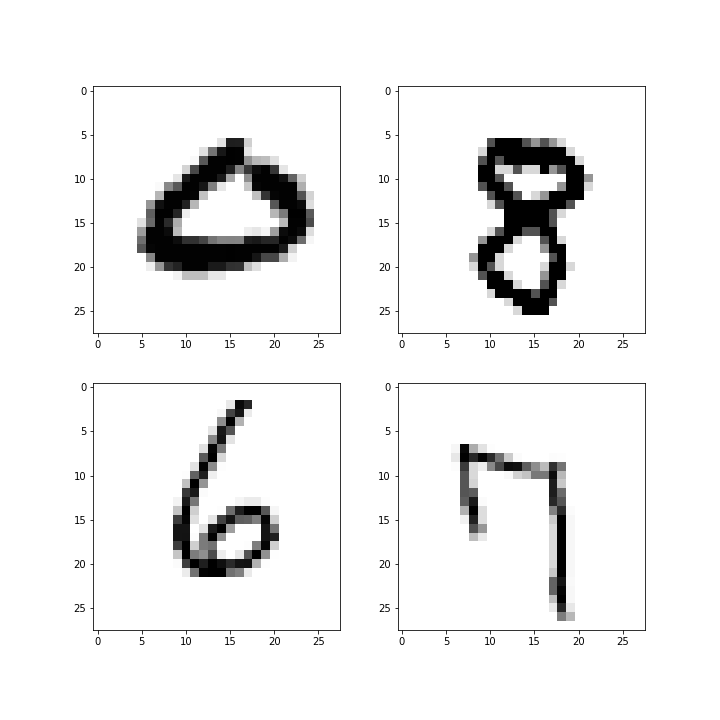
\includegraphics[width=1\linewidth]{MNISTExamples.png}
\end{subfigure}%
\begin{subfigure}{.6\textwidth}
  \centering
  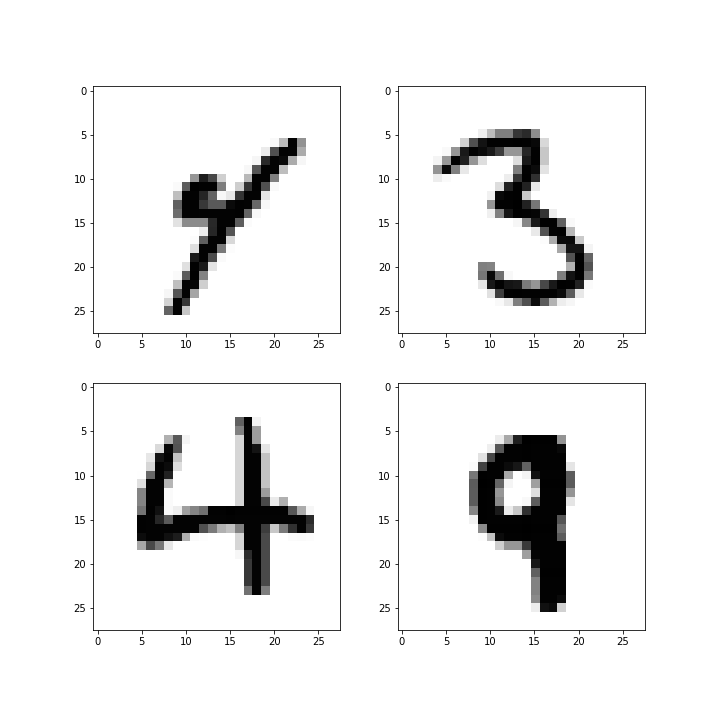
\includegraphics[width=1\linewidth]{MNISTExamples2.png}
\end{subfigure}
\caption{Sample figures from the MNIST dataset}
\label{fig:MNISTSamples}
\end{figure}
\subsection{CIFAR 10}\label{CIFAR10}
The CIFAR 10 dataset \cite{krizhevsky2009learning} is another image classification dataset; the inputs for each samples are 32x32x3 RGB colour pixel values (3 separate channels for the Red, Green and Blue colour value), while the labels specify the class of each image. The possible classes are `airplane', `automobile', `bird', `cat', `deer', `dog' ,'frog', `horse', `ship' and `truck'. As can be seen in Figure \ref{fig:CIFARSamples}, the images are significantly downsampled, resulting in images that can be difficult even for a human observer to classify, resulting in a significantly more difficult task than either MNIST or the Geometric Shapes database. For this dataset we use convolutional networks, as introduced in Section \ref{sec:convnets}, this will both improve the results of the experiments with CIFAR 10, but will also test the performance of the curriculum methods with a different type of network.

\begin{figure}[h!]
\hspace*{-2cm}    
\centering
\begin{subfigure}{.6\textwidth}
  \centering
  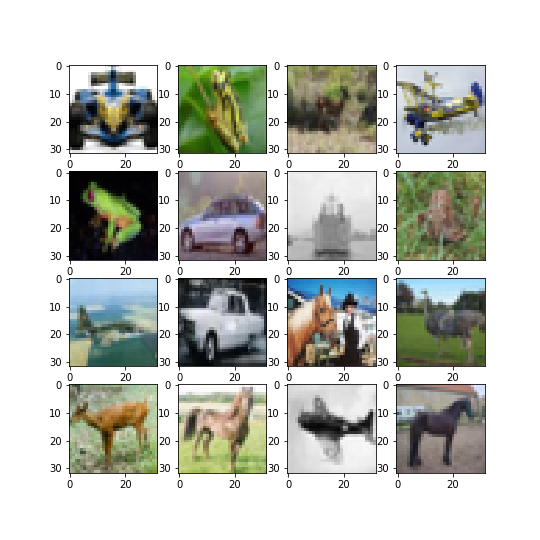
\includegraphics[width=1\linewidth]{CIFARExamples.png}
\end{subfigure}%
\begin{subfigure}{.6\textwidth}
  \centering
  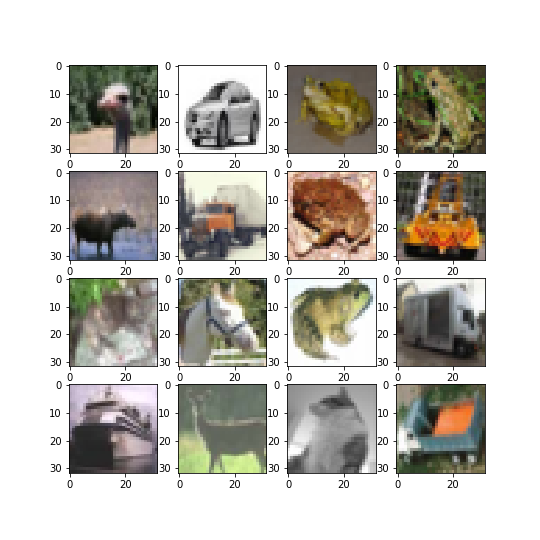
\includegraphics[width=1\linewidth]{CIFARExamples2.png}
\end{subfigure}
\caption{Sample figures from the CIFAR 10 dataset}
\label{fig:CIFARSamples}
\end{figure}



\section{Experiments}
We test the different dynamic curriculum methods introduced above on the Geometric Shapes, MNIST and CIFAR 10 image classification datasets, as introduced in Sections \ref{sec:GeoShapes}, \ref{MNIST} and \ref{CIFAR10}, respectively. For each dataset we used a validation set to construct an architecture and hyperparameters which achieved reasonable accuracies, then used those setting in the experiments for the different curriculum methods, the architectures for each dataset are laid out in Tables \ref{tab:GeoArchitecture2} to \ref{tab:CIFARArchitecture}. Note that in the case of CIFAR, the convolutional layer (denoted ``conv'') are following by a max pooling layer \cite{nagi2011max} and a batch normalization layer \cite{ioffe2015batch}, and ReLU denotes the Rectified Linear Unit activation function\cite{nair2010rectified}. 

\begin{table}[h!]
\caption{Geometric Shapes Dataset Model Architecture} \label{tab:GeoArchitecture2}
\begin{tabular}{|c||c|c|c|c|c|c|c|}
\hline
\multicolumn{8}{|c|}{Geometric Shapes Dataset Model Architecture} \\
\hline
 & Layer 1 & Layer 2 & Layer 3& Layer 4 &Layer 5 & Layer 6 & Layer 7 \\
\hline
\hline
Layer Type & FC & Dropout & FC & Dropout & FC & Dropout  & FC \\
\hline
Units & 300 & NA & 300 & NA & 300 & NA & 3 \\
\hline
Activation & Tanh & NA & Tanh & NA & Tanh & NA & Softmax \\
\hline
\end{tabular}
\end{table}

\begin{table}[h!]
\caption{MNIST Dataset Model Architecture} \label{tab:MNISTArchitecture}
\begin{tabular}{|c||c|c|c|c|c|c|c|}
\hline
\multicolumn{8}{|c|}{MNIST Dataset Model Architecture} \\
\hline
 & Layer 1 & Layer 2 & Layer 3& Layer 4 &Layer 5 & Layer 6 & Layer 7 \\
\hline
\hline
Layer Type & FC & Dropout & FC & Dropout & FC & Dropout  & FC \\
\hline
Units & 300 & NA & 300 & NA & 300 & NA & 3 \\
\hline
Activation & ReLU & NA & ReLU & NA & ReLU & NA & Softmax \\
\hline
\end{tabular}
\end{table}

\begin{table}[h!]
\caption{CIFAR Dataset Model Architecture} \label{tab:CIFARArchitecture}
\begin{tabular}{|c||c|c|c|c|c|c|c|}
\hline
\multicolumn{8}{|c|}{CIFAR Dataset Model Architecture} \\
\hline
 & Layer 1 & Layer 2 & Layer 3& Layer 4 &Layer 5 & Layer 6 & Layer 7 \\
\hline
\hline
Layer Type & Conv & Conv & Flatten & Dropout & FC & Dropout  & FC \\
\hline
Units & 50 & 50 & NA & NA & 100 & NA & 10 \\
\hline
Activation & ReLU &ReLU & NA & NA & ReLU & NA & Softmax \\
\hline
Kernel Size & 3x3 &3x3 & NA &NA &NA &NA &NA  \\
\hline
\end{tabular}
\end{table}

We run experiments across all three datasets using the curriculum methods laid out above, testing both `easy to hard' curricula and `hard to easy' curricula, as well as tested using different uncertainty functions. In each case we also train a baseline model trained without a curriculum to provide a comparison for the curriculum model test performances. We did not test all permutations of curricula and uncertainty functions as it became clear in some experiments that there was little difference from the baseline performance, the experiments for which we performed repeated tests and present results are as follows:
\begin{itemize}
\item Geometric Shapes, using the AADT uncertainty function:
\begin{itemize}
\item{Dynamic Task Curriculum, Easy to Hard}
\item{Dynamic Task Curriculum, Hard to Easy}
\item{Dynamic Sampling Curriculum, Hard to Easy}
\item{Dynamic Sampled Task Curriculum, Hard to Easy}
\item{Uniform Sampling Baseline}
\end{itemize}
\item MNIST, using the AADT uncertainty function:
\begin{itemize}
\item{Dynamic Task Curriculum, Easy to Hard}
\item{Dynamic Sampling Curriculum, Easy to Hard}
\item{Dynamic Sampled Task Curriculum, Easy to Hard}
\item{Dynamic Task Curriculum, Hard to Easy}
\item{Dynamic Sampling Curriculum, Hard to Easy}
\item{Dynamic Sampled Task Curriculum, Hard to Easy}
\item{Uniform Sampling Baseline}
\end{itemize}
\item CIFAR 10, using the BALD uncertainty function\footnote {Tests for CIFAR 10 with the AADT function resulted in little difference with from baseline, however using the BALD uncertainty function improved performance significantly.}:
\begin{itemize}
\item{Dynamic Task Curriculum, Easy to Hard}
\item{Dynamic Sampled Task Curriculum, Easy to Hard}
\item{Dynamic Task Curriculum, Hard to Easy}
\item{Dynamic Sampled Task Curriculum, Hard to Easy}
\item{Uniform Sampling Baseline}
\end{itemize}
\end{itemize}
\begin{table}[h!]
\caption{Experiment Hyperparameters} \label{tab:HyperParams2}
\hspace*{-2cm}
\begin{tabular}{|c||c|c|c|c|c|c|c|}
\hline
\multicolumn{7}{|c|}{Experiment Hyperparameters} \\
\hline
 &Epochs & Optimiser &Learning Rate & Dropout \% & Batch Size & Num Tasks\\
\hline
Geometric Shapes & 350 & Adam & 0.0001 & 0.25 & 32 & 2  \\
\hline
MNIST & 50 & Adam & 0.0001 & 0.25 & 50 & 2  \\
\hline
CIFAR 10 & 50 & Adam & 0.0001 & 0.25 & 100 & 2  \\
\hline
\end{tabular}
\end{table}
We run the experiments 10 times with different random initialistions, reporting average results and standard errors. In Table \ref{tab:HyperParams2} we lay out the other hyperparameters for the experiments. Note that in each case we keep the number of tasks at 2; results were robust to differing the number of tasks however as we did not have time to do a full analysis we decided to keep the experimental setups relatively homogeneous in order to avoid tinkering with hyperparameters to achieve positive results. As in Chapter \ref{ch:BootstrappedActiveCurricula}, experiments were carried out in Keras \cite{chollet2015keras} and the Adam optimiser is implemented with the default hyperparameters (except for the learning rate which is given in Table \ref{tab:HyperParams2}). 

\section{Results and Discussion}
The results for  the experiments are  illustrated in Figures \ref{fig:GeoShapesDACResults} and \ref{fig:DACResults}\footnote{Due to the experimental setup for the CIFAR 10 experiments, only test accuracies were recorded.}, full results are detailed in Tables \ref{tab:GeoShapes DACResults} to \ref{tab:CIFAR DACResults}. Note that the denotation `easy' implies that the curriculum was trained on an easy to hard curriculum, with increasingly difficult tasks in the DTC case and by biasing sampling towards easy samples in the DSC method, and similarly for the DSTC method. Conversely, `Hard' denotes that the curriculum used was a hard to easy curriculum.

\begin{figure}[h!]
\hspace*{-3cm}    
\centering
\begin{subfigure}{0.7\textwidth}
  \centering
  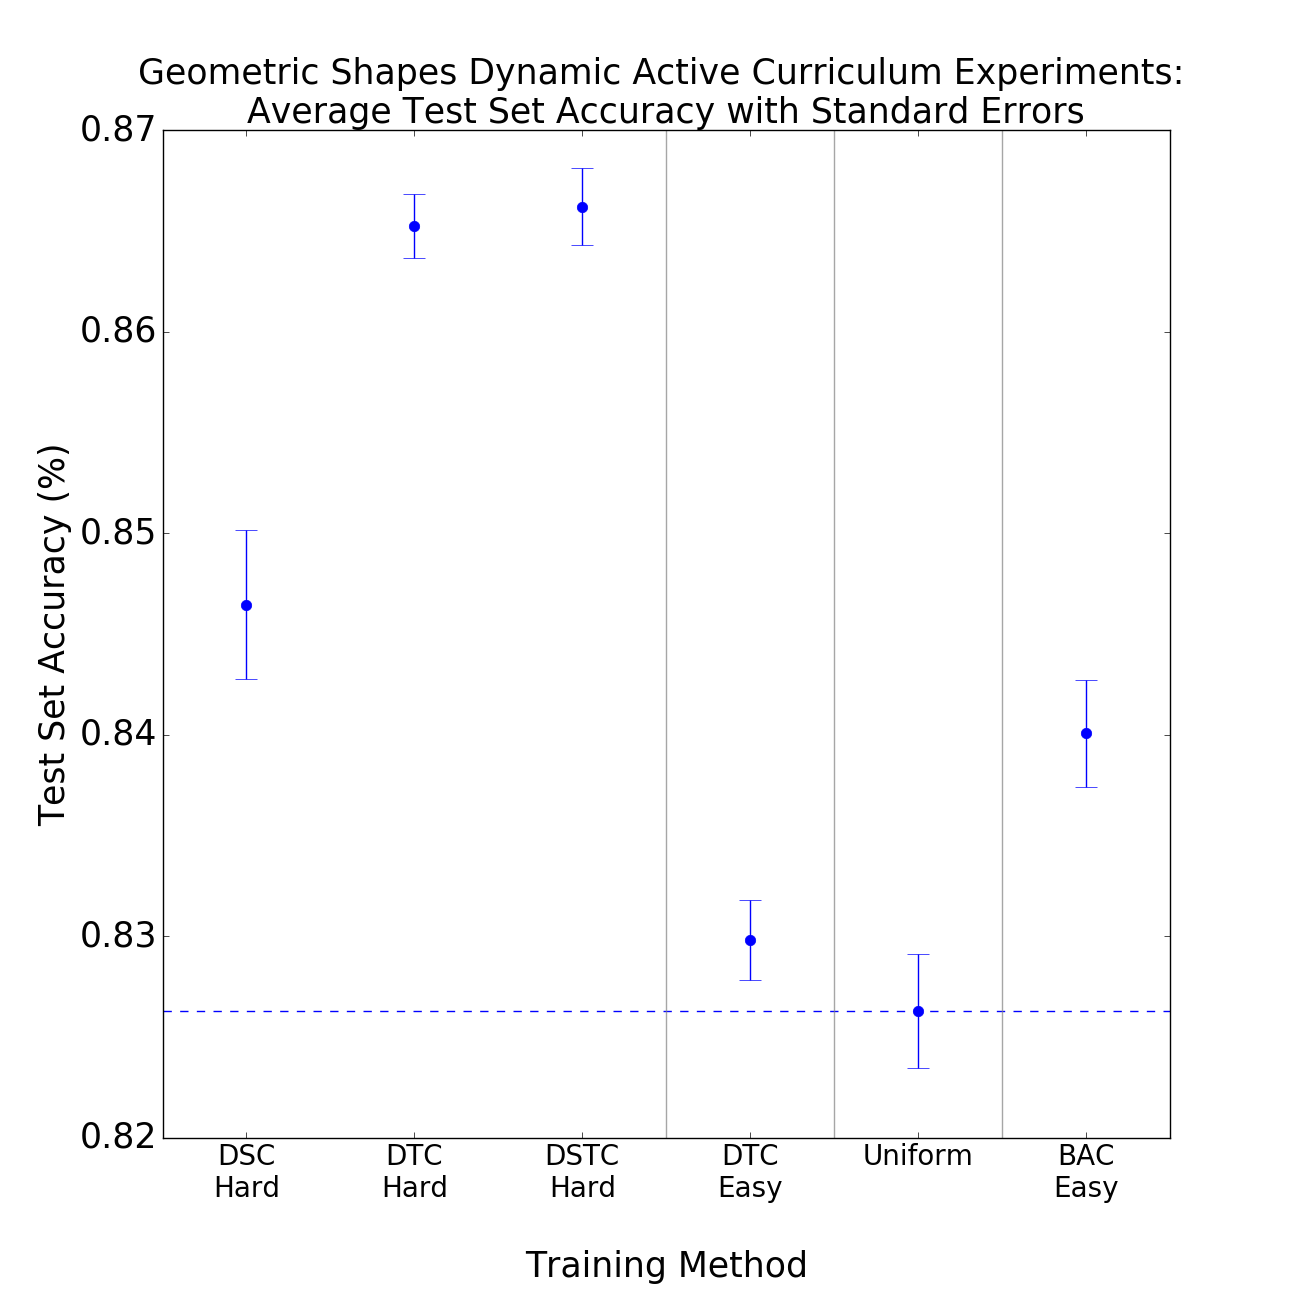
\includegraphics[width=1\linewidth]{GeoShapes_Dynamic_Results_STE.png}
  \caption{ Mean Test Set Accuracies}
  \label{fig:DAC_ste_Geo}
\end{subfigure}%
\begin{subfigure}{0.7\textwidth}
\hspace*{-1cm}   
  \centering
  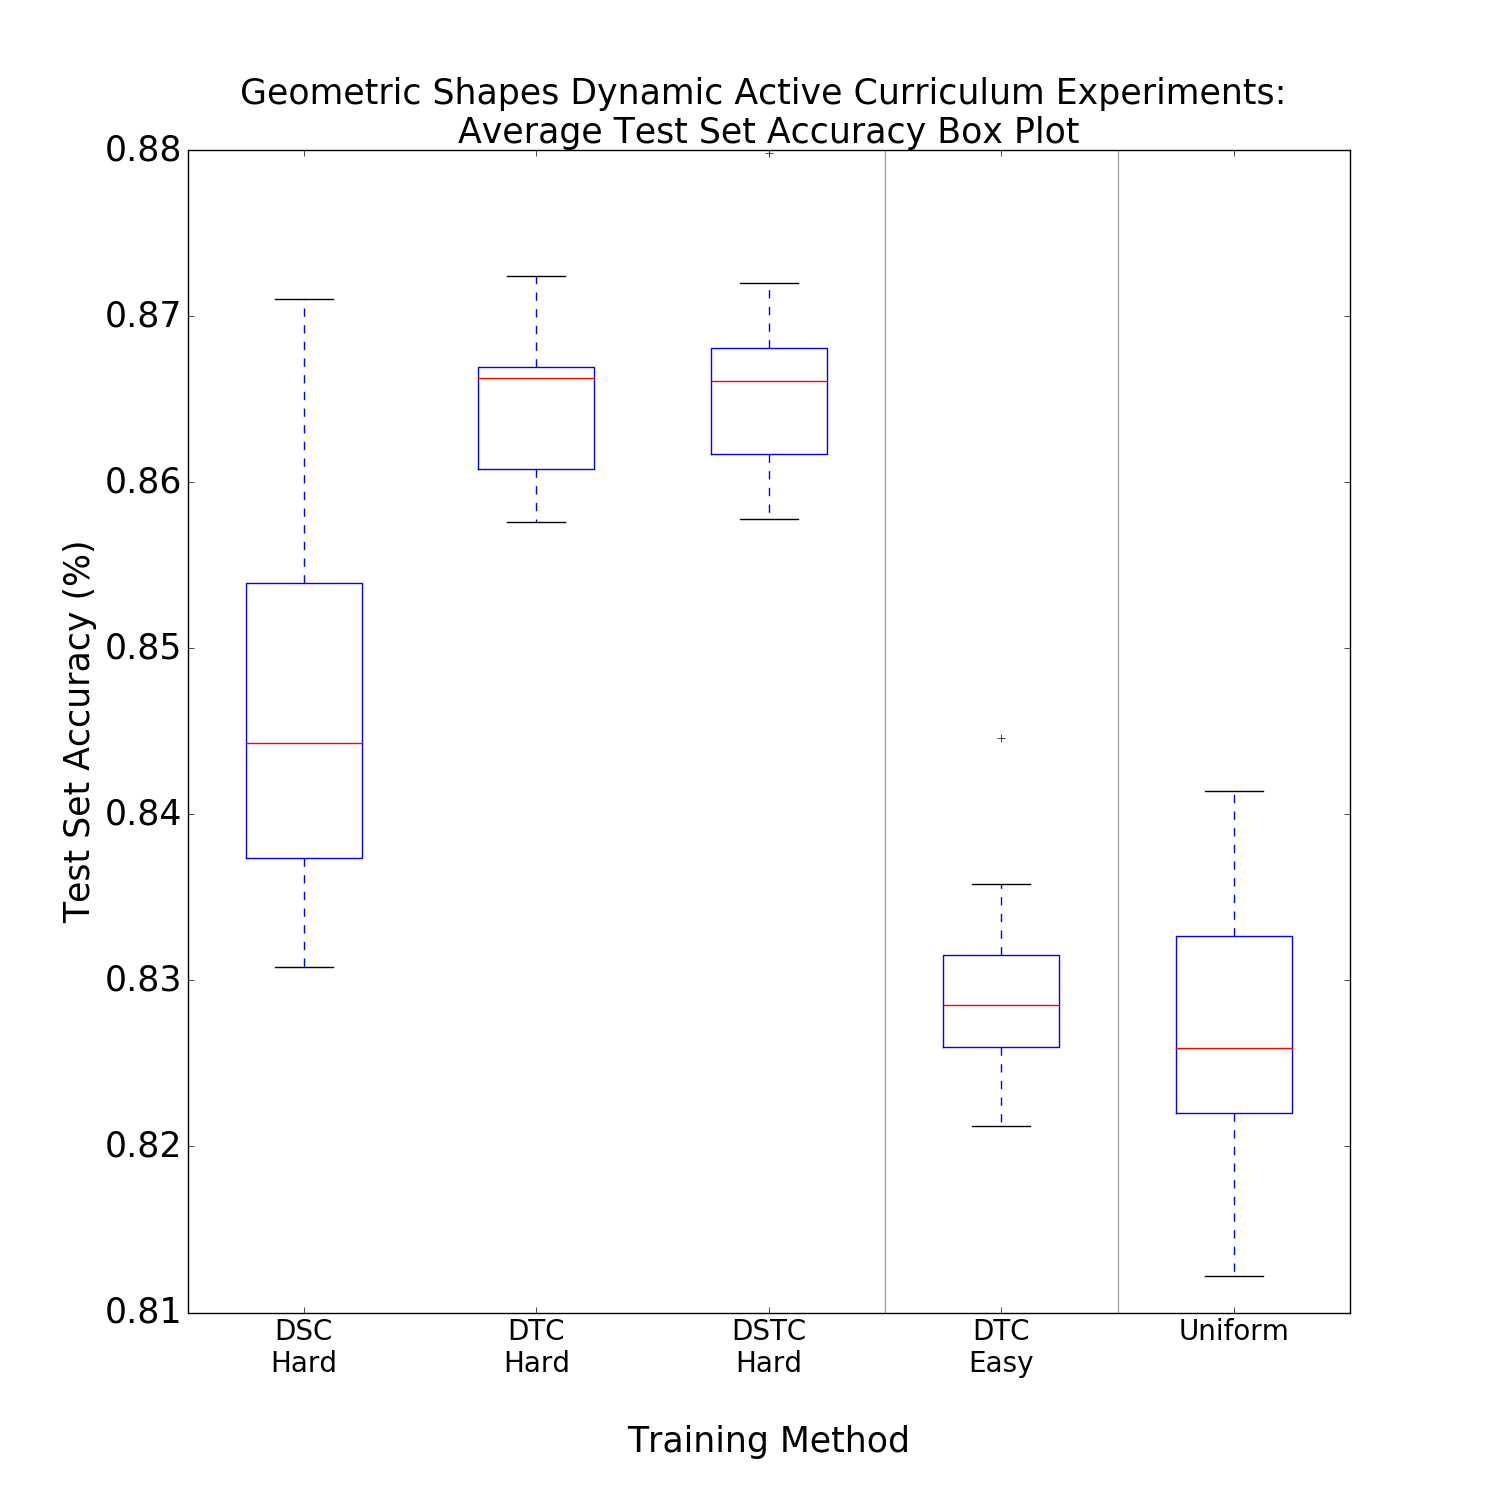
\includegraphics[width=1\linewidth]{GeoShapes_Dynamic_Results_Boxplt.png}
  \caption{Test Set Accuracy Boxplots}
  \label{fig:DAC_BoxPlt_Geo}
\end{subfigure}
\caption{Geometric Shapes Dynamic Active Curriculum (DAC) Experiment Results}
\label{fig:GeoShapesDACResults}
\end{figure}

The Geometric Shapes results shows a significant increase in test performance, particularly for the 'hard' curriculum models, where the model is trained on increasingly easy samples, contrary to the usual curriculum learning approach and more in line with an active learning philosophy on sample selection. All three 'hard' curriculum construction methods outperformed the benchmark, and, as shown in Figure \ref{fig:DAC_ste_Geo}, also significantly outperformed the bootstrapped active curriculum approach from Chapter \ref{ch:BootstrappedActiveCurricula}. Nevertheless, the more traditional 'easy' curriculum method also outperformed the benchmark in the DTC case, although it underperformed the BAC test performance, and the `easy' sampling based dynamic curriculum methods did not lead to significantly different results to the uniform baseline model (not shown here). 

\begin{figure}[h!]
\hspace*{-1.5cm}    
\centering
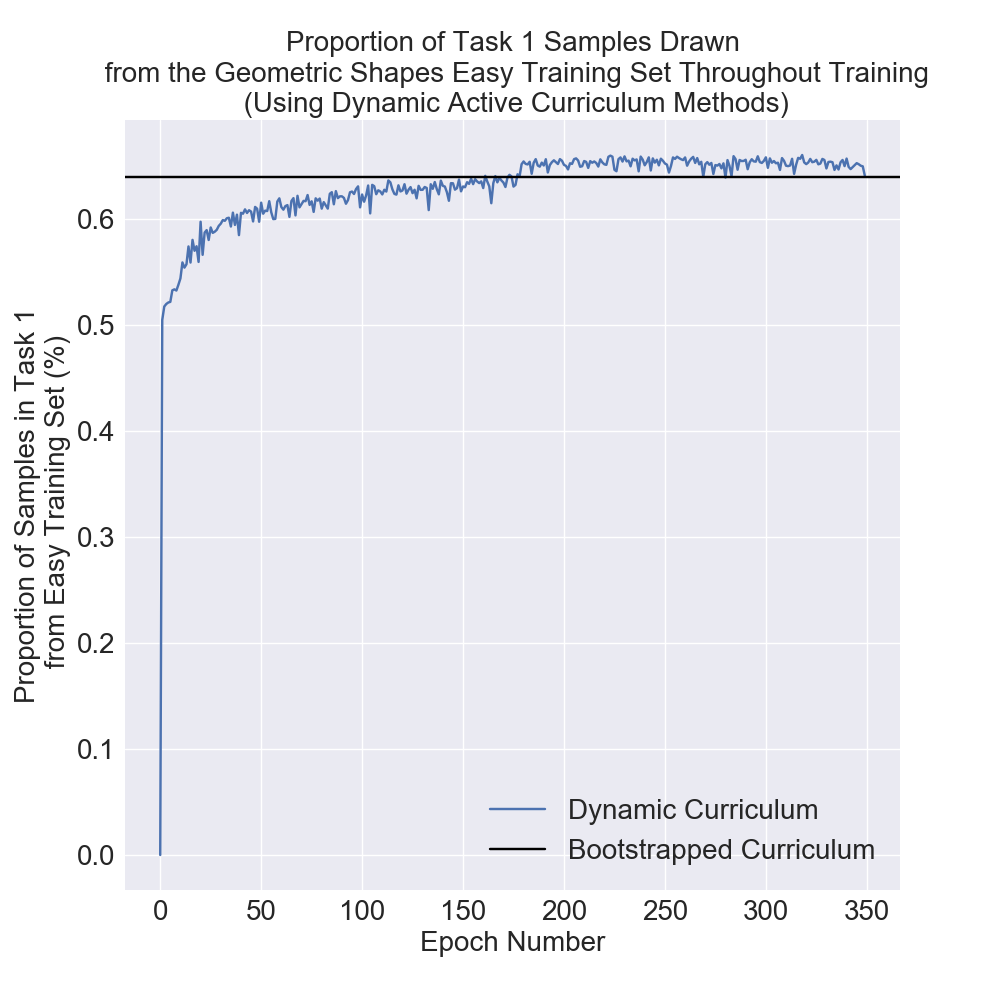
\includegraphics[width=0.92\linewidth]{DAC_GeoShapes_Proportion.png}
\caption{Analysis of the proportion of samples from the construct 'easy' first tasks of the dynamic active curricula taken from the easy Geometric Shapes training data.}
\label{fig:GeoShapes_DAC_Prop}
\end{figure}


Analysing the curriculum methods throughout training provides some insights into how the dynamic curricula choose training samples. As discussed in Section \ref{sec:GeoShapes}, the Geometric Shapes training data is made of up an 'easy' training set of regular shapes and a 'hard' training set of more general shapes. We can see from monitoring the output of the uncertainty function throughout training that the model can quickly starts to discriminate between the hard and easy training set, with the first task constructed at the start of each epoch of the easy dynamic task curriculum quickly becoming biased towards samples from the easy training set, suggesting that one does not need to fully train a baseline model, as in the bootstrapped curriculum method, to be able to approximate the relative difficulty of the training samples. Indeed, the proportion of the first, easier task coming from the easy training set throughout training quickly converges and ultimately exceeds the proportion in the easy task of the boostrapped curriculum method, where the model used to measure uncertainty is fully trained, as illustrated in Figure \ref{fig:GeoShapes_DAC_Prop}. This result is slightly confounding however, as it does not explain why the hard to easy versions of the dynamic active curricula achieve much higher test performances than the easy to hard methods, given that the dynamic curricula seem to ranking the samples in similar ways, yet the hard to easy boostrapped curriculum method underperformed even the baseline model. 



\begin{figure}[h!]
\hspace*{-3cm}    
\centering
\begin{subfigure}{0.7\textwidth}
  \centering
  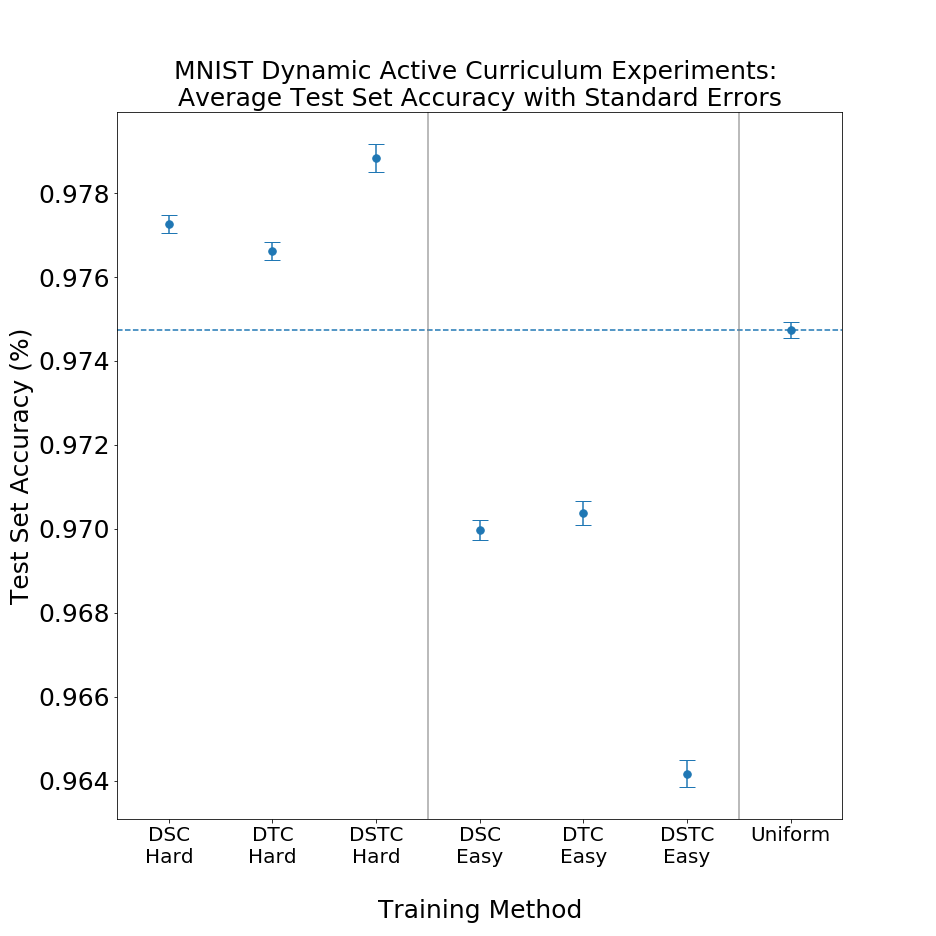
\includegraphics[width=1\linewidth]{MNIST_Dynamic_Results.png}
  \caption{ Mean Test Set Accuracies}
  \label{fig:DAC_ste_MNIST}
\end{subfigure}%
\begin{subfigure}{0.7\textwidth}
\hspace*{-1cm}   
  \centering
  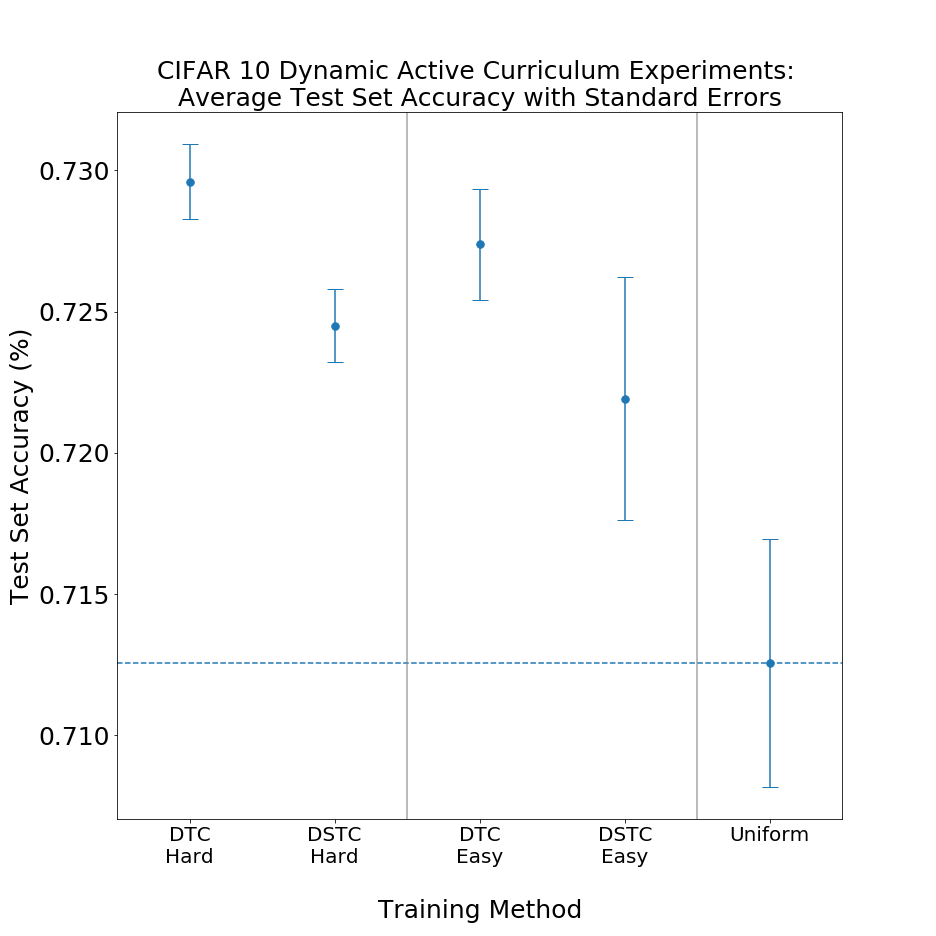
\includegraphics[width=1\linewidth]{CIFAR_Dynamic_Results.png}
  \caption{Test Set Accuracy Boxplots}
  \label{fig:DAC_ste_CIFAR}
\end{subfigure}
\caption{MNIST and CIFAR 10 Dynamic Active Curriculum (DAC) Experiment Results}
\label{fig:DACResults}
\end{figure}


Figure \ref{fig:DAC_ste_MNIST} shows the performance of the curriculum methods for the MNIST dataset; as in the case of Geometric Shapes, the best performing curriculum is the hard to easy dynamic sampled task curriculum, combining the dynamic task based approach with the biased sampling methodology. While the outperformance in the case of MNIST is fairly small on an absolute basis (the best performing model achieving an average test accuracy only 0.4\% higher than the baseline model), given the relatively high overall accuracy achievable on the MNIST dataset this might be considered significant, particularly given the consistency in the results illustrated by the standard error bars. Unlike in the Geometric Shapes results however, the MNIST test accuracies for the easy to hard curricula are significantly lower than the baseline. One hypothesis for explaining this is that emphasising easy samples may be most effective in the early stages of training when the model is still poorly calibrated on the task. In the case of MNIST however, validation accuracy can exceed 90\% after only a single training epoch, suggesting that it is such a simple task that an easy to hard curriculum would not be beneficial, and that it would be better to focus training on difficult samples instead, explaining the performance of the hard to easy curriculum methods. This dynamic is also suggested in \cite{Chang18} and \cite{weinshall2018curriculum}, where it is suggested that the efficacy of curriculum learning may be related to the difficulty of the task, relative to the capacity of the network. We attempted to test this hypothesis by repeating the experiments with a 'noisy' version of the MNIST dataset, where the input images are corrupted with increasing levels of random noise; while we did not find any variation in the relative order of test accuracies shown in Figure \ref{fig:DAC_ste_MNIST}, we did notice that the model was still able to achieve high levels of accuracy on the validation set very early in training, suggesting that the noise adding procedure was ineffective and that perhaps different data augmentation techniques would be better suited to 
testing this hypothesis. 

\begin{figure}[h!]
\hspace*{-3cm}    
\centering
\begin{subfigure}{0.7\textwidth}
  \centering
  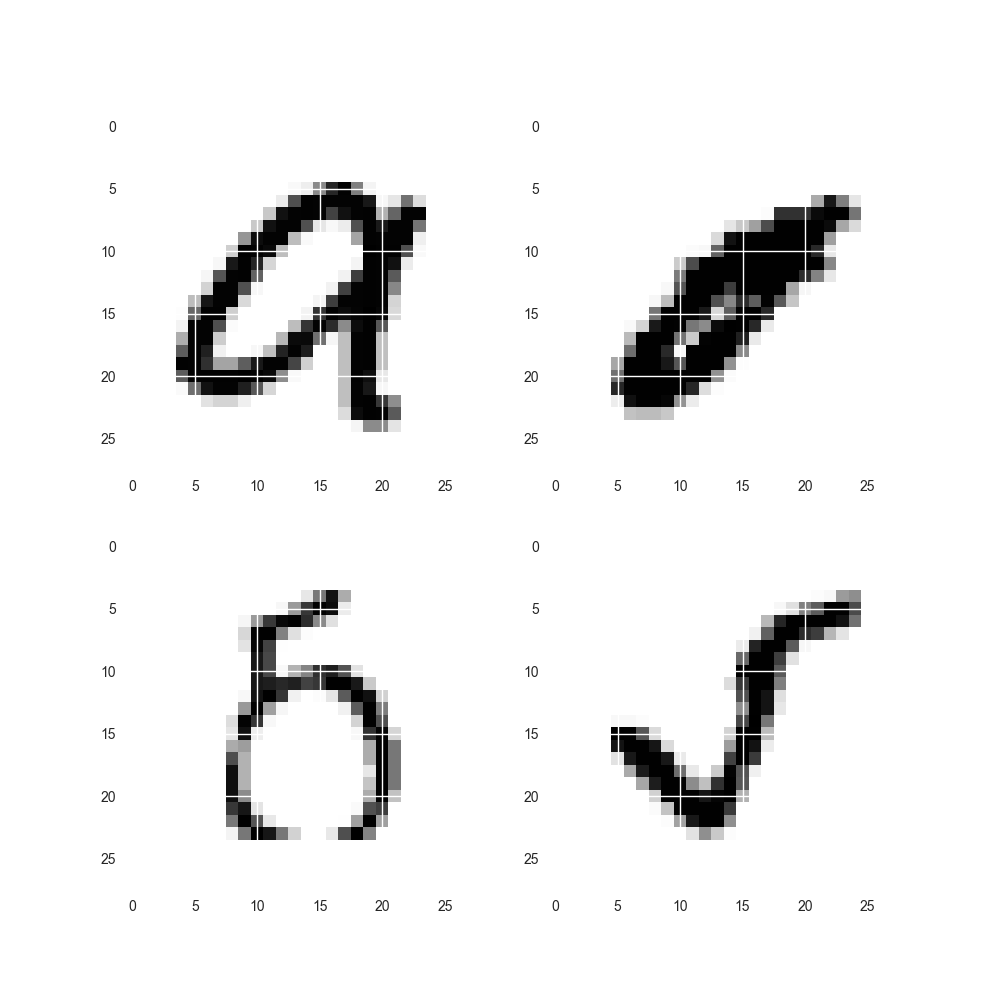
\includegraphics[width=1\linewidth]{MNIST_Uncertain_Samples.png}
  \caption{4 Most Uncertain MNIST Samples}
  \label{fig:MNIST_Uncertain}
\end{subfigure}%
\begin{subfigure}{0.7\textwidth}
\hspace*{-1cm}   
  \centering
  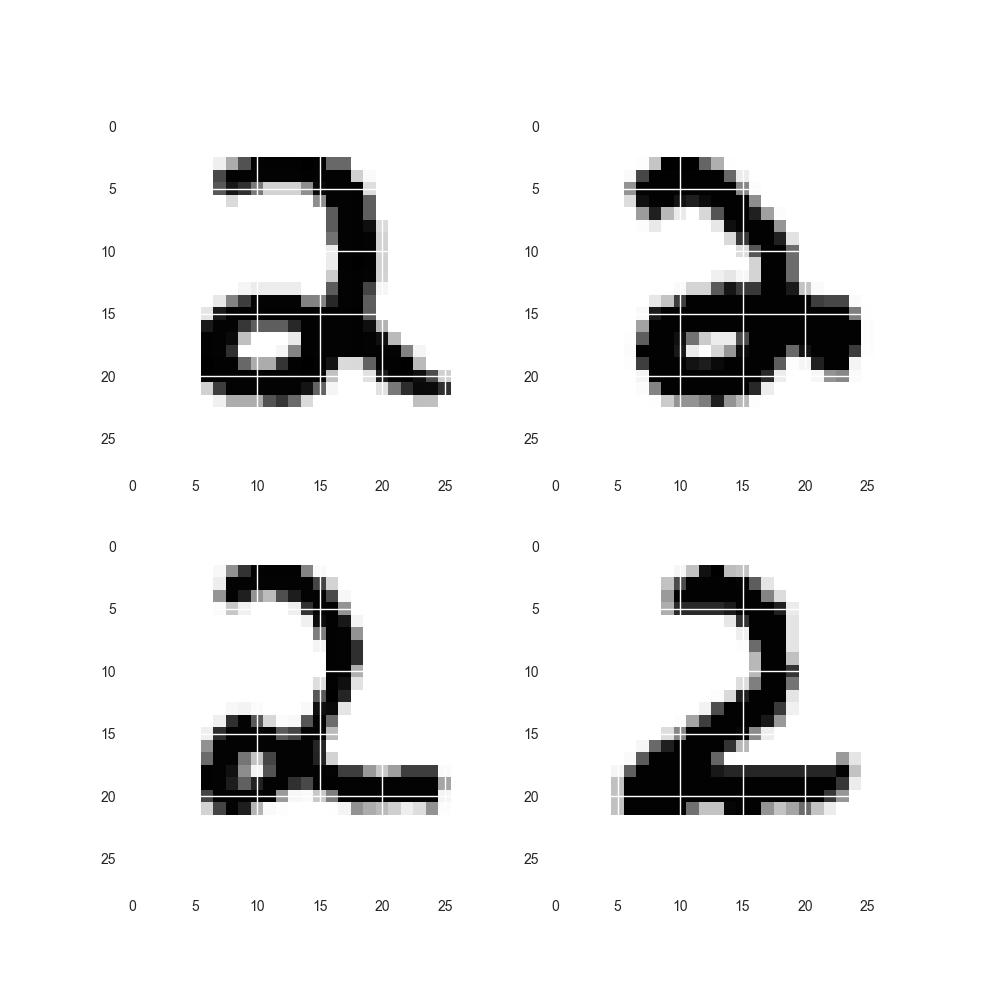
\includegraphics[width=1\linewidth]{MNIST_certain_Samples.png}
  \caption{4 Least Uncertain MNIST Samples}
  \label{fig:MNIST Certain}
\end{subfigure}
\caption{Top 4 most/least uncertain training samples from the MNIST dataset using a dynamic curriculum model.}
\label{fig:MNISTSampleUncertainty}
\end{figure}


While there is not a clear delineation of difficulty in the MNIST dataset, examining the model uncertainty for the training set reveals that the method does appear to be effective at identifying samples that correspond to an intuitive sense of difficulty. Figure \ref{fig:MNIST_Uncertain} shows the samples that one of the curriculum models was most uncertain about classifying (at the end of training), while Figure \ref{fig:MNIST Certain} shows the samples the model was most certain about classifying. Figure \ref{fig:MNIST Certain} clearly shows that the model is most confident in classifying the number 2, while \ref{fig:MNIST_Uncertain} illustrates the irregularity of the samples that the model is uncertain in classifying, with some samples not even appearing to be numbers. This analysis would suggest that using an active learning inspired uncertainty metric is an effective way of automatically inferring sample difficulty, even when done dynamically whilst training the model. Furthermore the outperformance of the curriculum methods would suggest that these uncertainty measures can effectively be used to construct a learning curriculum.

\begin{figure}[h!]
\hspace*{-3cm}    
\centering
\begin{subfigure}{0.7\textwidth}
  \centering
  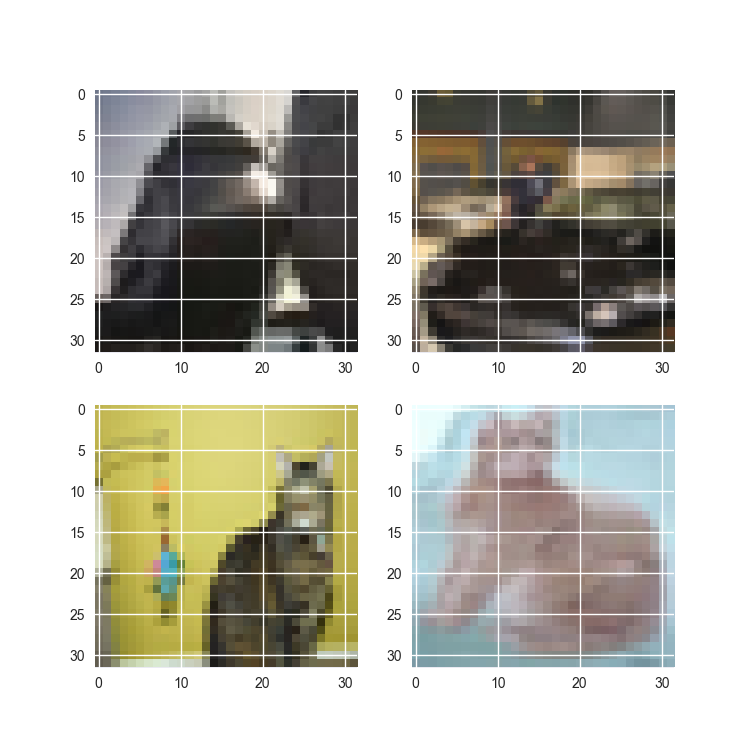
\includegraphics[width=1\linewidth]{CIFAR_Uncertain_Samples.png}
  \caption{4 Most Uncertain CIFAR Samples (BALD)}
  \label{fig:CIFAR_Uncertain}
\end{subfigure}%
\begin{subfigure}{0.7\textwidth}
\hspace*{-1cm}   
  \centering
  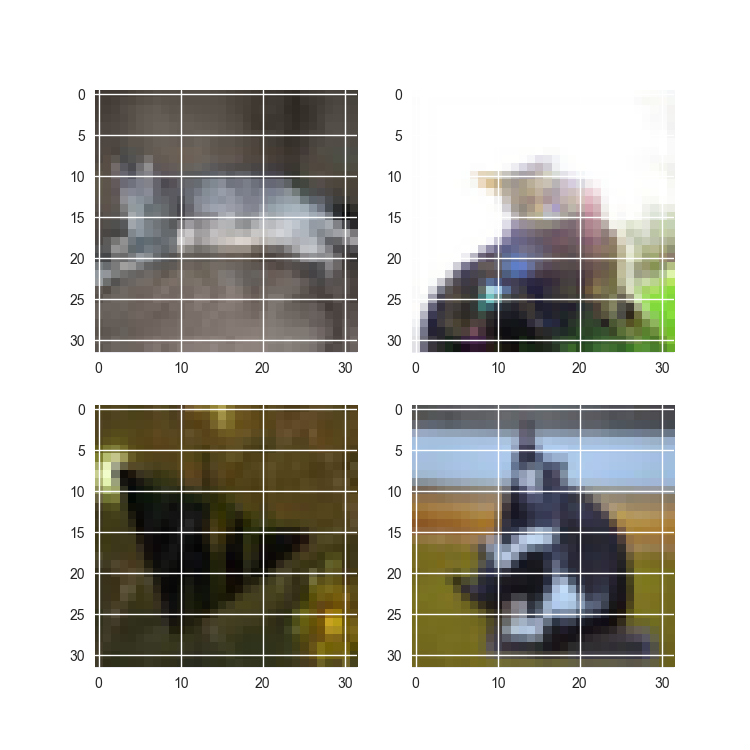
\includegraphics[width=1\linewidth]{CIFAR_certain_Samples.png}
  \caption{4 Least Uncertain CIFAR Samples (BALD)}
  \label{fig:CIFAR Certain}
\end{subfigure}
\caption{Top 4 most/least uncertain training samples from the CIFAR dataset using a dynamic curriculum model (BALD uncertainty function).}
\label{fig:CIFARSampleUncertainty}
\end{figure}

Figure \ref{fig:DACResults} shows the results for the CIFAR 10 dataset, using the BALD activation function detailed in Section \ref{BALD}. Interestingly, both the easy to hard and hard to easy dynamic curriculum methods consistently exceeded the benchmark test accuracy, with the best performing curriculum method being the hard to easy DTC method which improved on the test accuracy by an average of 1.7\%. Unlike with MNIST and Geometric Shapes however, in both cases adding the sampling component and sampling from the tasks proportionally to uncertainty inhibited performance, with the best performance in both the hard to easy and easy to hard case coming from the purely task based dynamic curricula. The fact that both the easy to hard and hard to easy curricula outperformed significantly in the case of CIFAR 10 is an interesting result, supporting the idea that beginning training with easy samples is most beneficial for 'difficult' problems. How one defines whether or not an entire dataset is difficult however, and is of course relative to the capacity of the learning algorithm. Nevertheless, simply based on test accuracy and training progression, CIFAR 10 would appear to be a more difficult task than learning on either the MNIST or Geometric Shapes datasets, supporting the suggestion in \cite{Chang18} and \cite{weinshall2018curriculum} that the effectiveness of curriculum methods is affected by the difficulty of the tasks. As with with the MNIST dataset there is no predefined curriculum for the CIFAR 10 dataset, however we can again analyse one of the trained models' classification uncertainty over the training set. Figure \ref{fig:CIFARSampleUncertainty} illustrates the four most and least uncertain samples at the end of one of the dynamic curriculum training runs, using the BALD uncertainty function. Unlike in the Geometric Shapes and MNIST datasets, the results are less intuitive; while the top two samples of Figure \ref{fig:CIFAR_Uncertain} do appear to be difficult to classify visually, the bottom two samples are clearly of the class `cat'. Similarly while some of the least uncertain samples shown in Figure \ref{fig:CIFAR Certain} appear to be 'easy' samples, insofar as the class labels seem obvious, the bottom two images are less clearly easy. 
\begin{figure}[h!]
\hspace*{-3cm}    
\centering
\begin{subfigure}{0.7\textwidth}
  \centering
  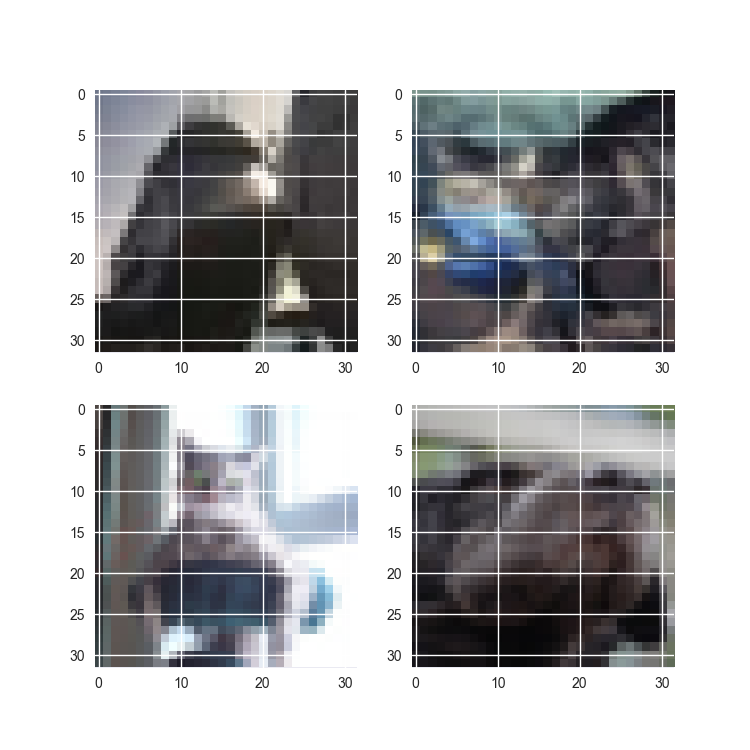
\includegraphics[width=1\linewidth]{CIFAR_certain_Samples_D2T.png}
  \caption{4 Most Uncertain CIFAR Samples (AADT)}
  \label{fig:CIFAR_Uncertain AADT}
\end{subfigure}%
\begin{subfigure}{0.7\textwidth}
\hspace*{-1cm}   
  \centering
  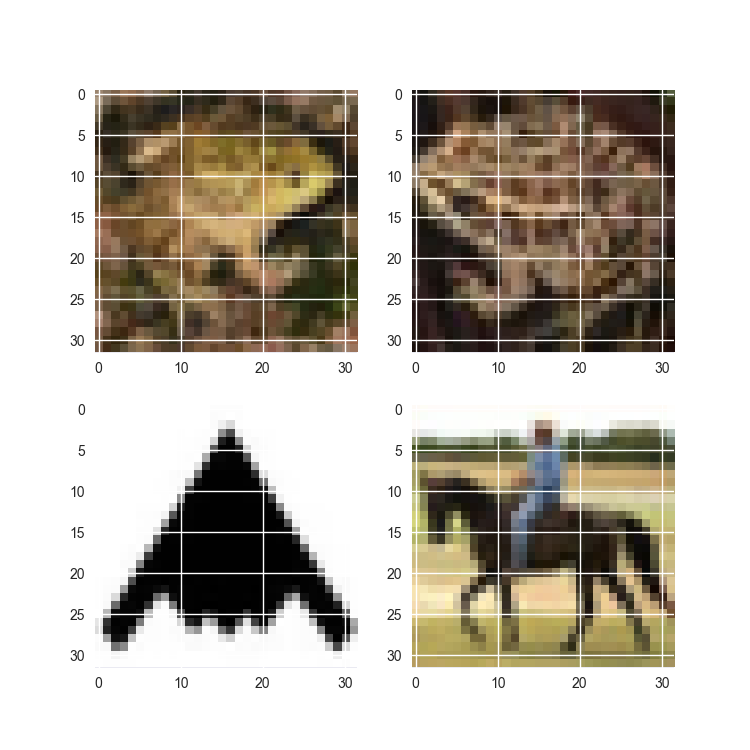
\includegraphics[width=1\linewidth]{CIFAR_Uncertain_Samples_D2T.png}
  \caption{4 Least Uncertain CIFAR Samples (AADT)}
  \label{fig:CIFAR Certain AADT}
\end{subfigure}
\caption{Top 4 most/least uncertain training samples from the CIFAR dataset using a dynamic curriculum model (AADT uncertainty function).}
\label{fig:CIFARSampleUncertaintyAADT}
\end{figure}
This may be the result of using the BALD uncertainty function, which gives an arguably more abstract definition of uncertainty than the distance to classification threshold method. Indeed, repeating the exercise with the AADT uncertainty function (\ref{BAC_AADT}), gives a slightly more intuitive result, as shown in Figure \ref{fig:CIFARSampleUncertaintyAADT}. Interestingly, the most uncertain image (the top left image in Figures \ref{fig:CIFAR_Uncertain} and \ref{fig:CIFAR_Uncertain AADT} are the same, suggesting some overlap between the uncertainty measures. However the least uncertain images using the AADT function seem to correspond much more to an intuitive sense of difficulty compared to the BALD function, with the bottom two images of Figure \ref{fig:CIFAR Certain AADT} clearly belonging to the 'Airplane' and 'Horse' classes. Nevertheless, the experiments with the AADT uncertainty with the CIFAR 10 dataset did not produce results significantly different to the baseline model, whereas using the BALD method led to consistently higher test accuracy. This might be seen to support the findings in Chapter \ref{ch:BootstrappedActiveCurricula} that even if we had a predefined curriculum according to a manual interpretation of sample difficulty, it may still be preferable to use an automated curriculum method that uses information from the model being trained to infer sample difficulty, such as those laid out in this paper. 

To conclude, the experiments carried out show promising results that the dynamic approach of curriculum construction can lead to improved model generalization, outperforming the more costly `boostrapped' curriculum approach laid out in Chapter \ref{ch:BootstrappedActiveCurricula}. Moreover, the dynamic active curriculum approach offers a novel and relatively simple way of potentially improving model performance, requiring changes to the standard deep model learning procedure that can be implemented with most deep learning software. More research is needed into which curriculum method is most appropriate for a given dataset, for example questions remain over which uncertainty function leads to the best results and whether or not an easy to hard or hard to easy curriculum is most appropriate. We develop these questions, as well as other suggestions for future research directions in the next chapter.




